\section{Appendix}

\subsection*{Merkle Tree}

Merkle Tree is a tree-like data structure in cryptography and computer science. Each leaf node uses the hash of the data block as a label, and nodes other than the leaf node use the cryptographic hash of its child node's label as the label. Hash trees can efficiently and securely verify the contents of large data structures.

Hash trees can be used to verify any type of data that is stored, processed, and transmitted from a computer to another. They can help ensure that data blocks received from other peers in the peer-to-peer network are not corrupted and altered, and even check if other peers are lying and sending fake data blocks.

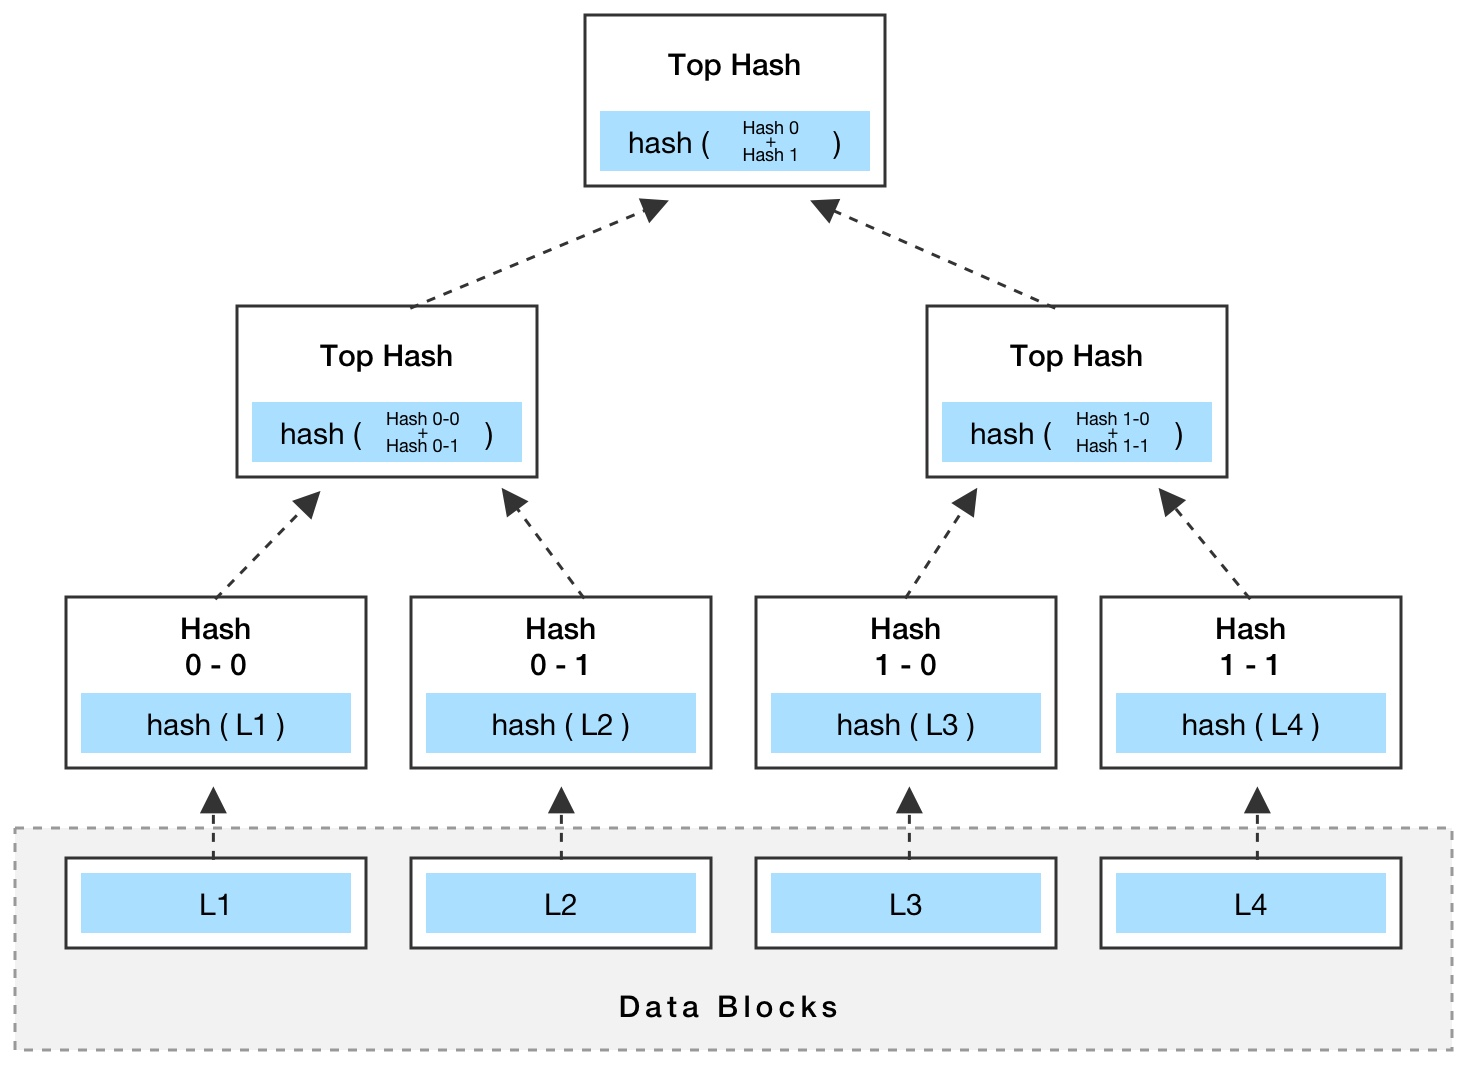
\includegraphics[scale=0.2]{pic/Merkle Tree.jpg}

\subsubsection{Definition (Collision resistant hash function)}

Collision resistance is a property of cryptographic hash functions: a hash function H is collision resistant if it is hard to find two inputs that hash to the same output; that is, two inputs a and b such that H(a) = H(b), and a $\ne $b\cite{CR}.

\subsubsection{Definition (Merkle Tree)}

A Merkle tree is a balanced binary tree, where each leaf node stores some value, and each non-leaf node holds the value $H(LeftChild||RightChild)$, where H is a collision-resistant hash function. The Balanced binary tree here means a tree with n leaves that has a depth less than or equal to $log_2(n)$.

\subsubsection{Definition (Merkle Proof)}

Given a Merkle tree, MT, with root r, a Merkle proof that x is the kth node in MT, $\Pi k\in MT$, are the siblings of each node on the path from x to r. Since MT has depth at most $log_2(n)$, the proof length is at most$log_2(n) + 1$ as each node in the path can be calculated from its two children so we only need the siblings and the 2 leaf nodes.

\begin{theorem}
(Soundness of Merkle-proofs). Given a Merkle tree, MT built using a collision-resistant hash function (Definition 8), a polynomial-time adversary cannot produce a valid proof $\Pi k\in MT$, for a k not in MT. 

\end{theorem}



\begin{theorem}
(Completeness of Merkle proofs) Given a Merkle tree built using a collision-resistant hash function, MT, and a node $k \in MT$, a polynomial-time adversary cannot generate a proof $\Pi k\in MT$ that is not a true path in MT. 
\end{theorem}



\begin{wrapfigure*}
\centering
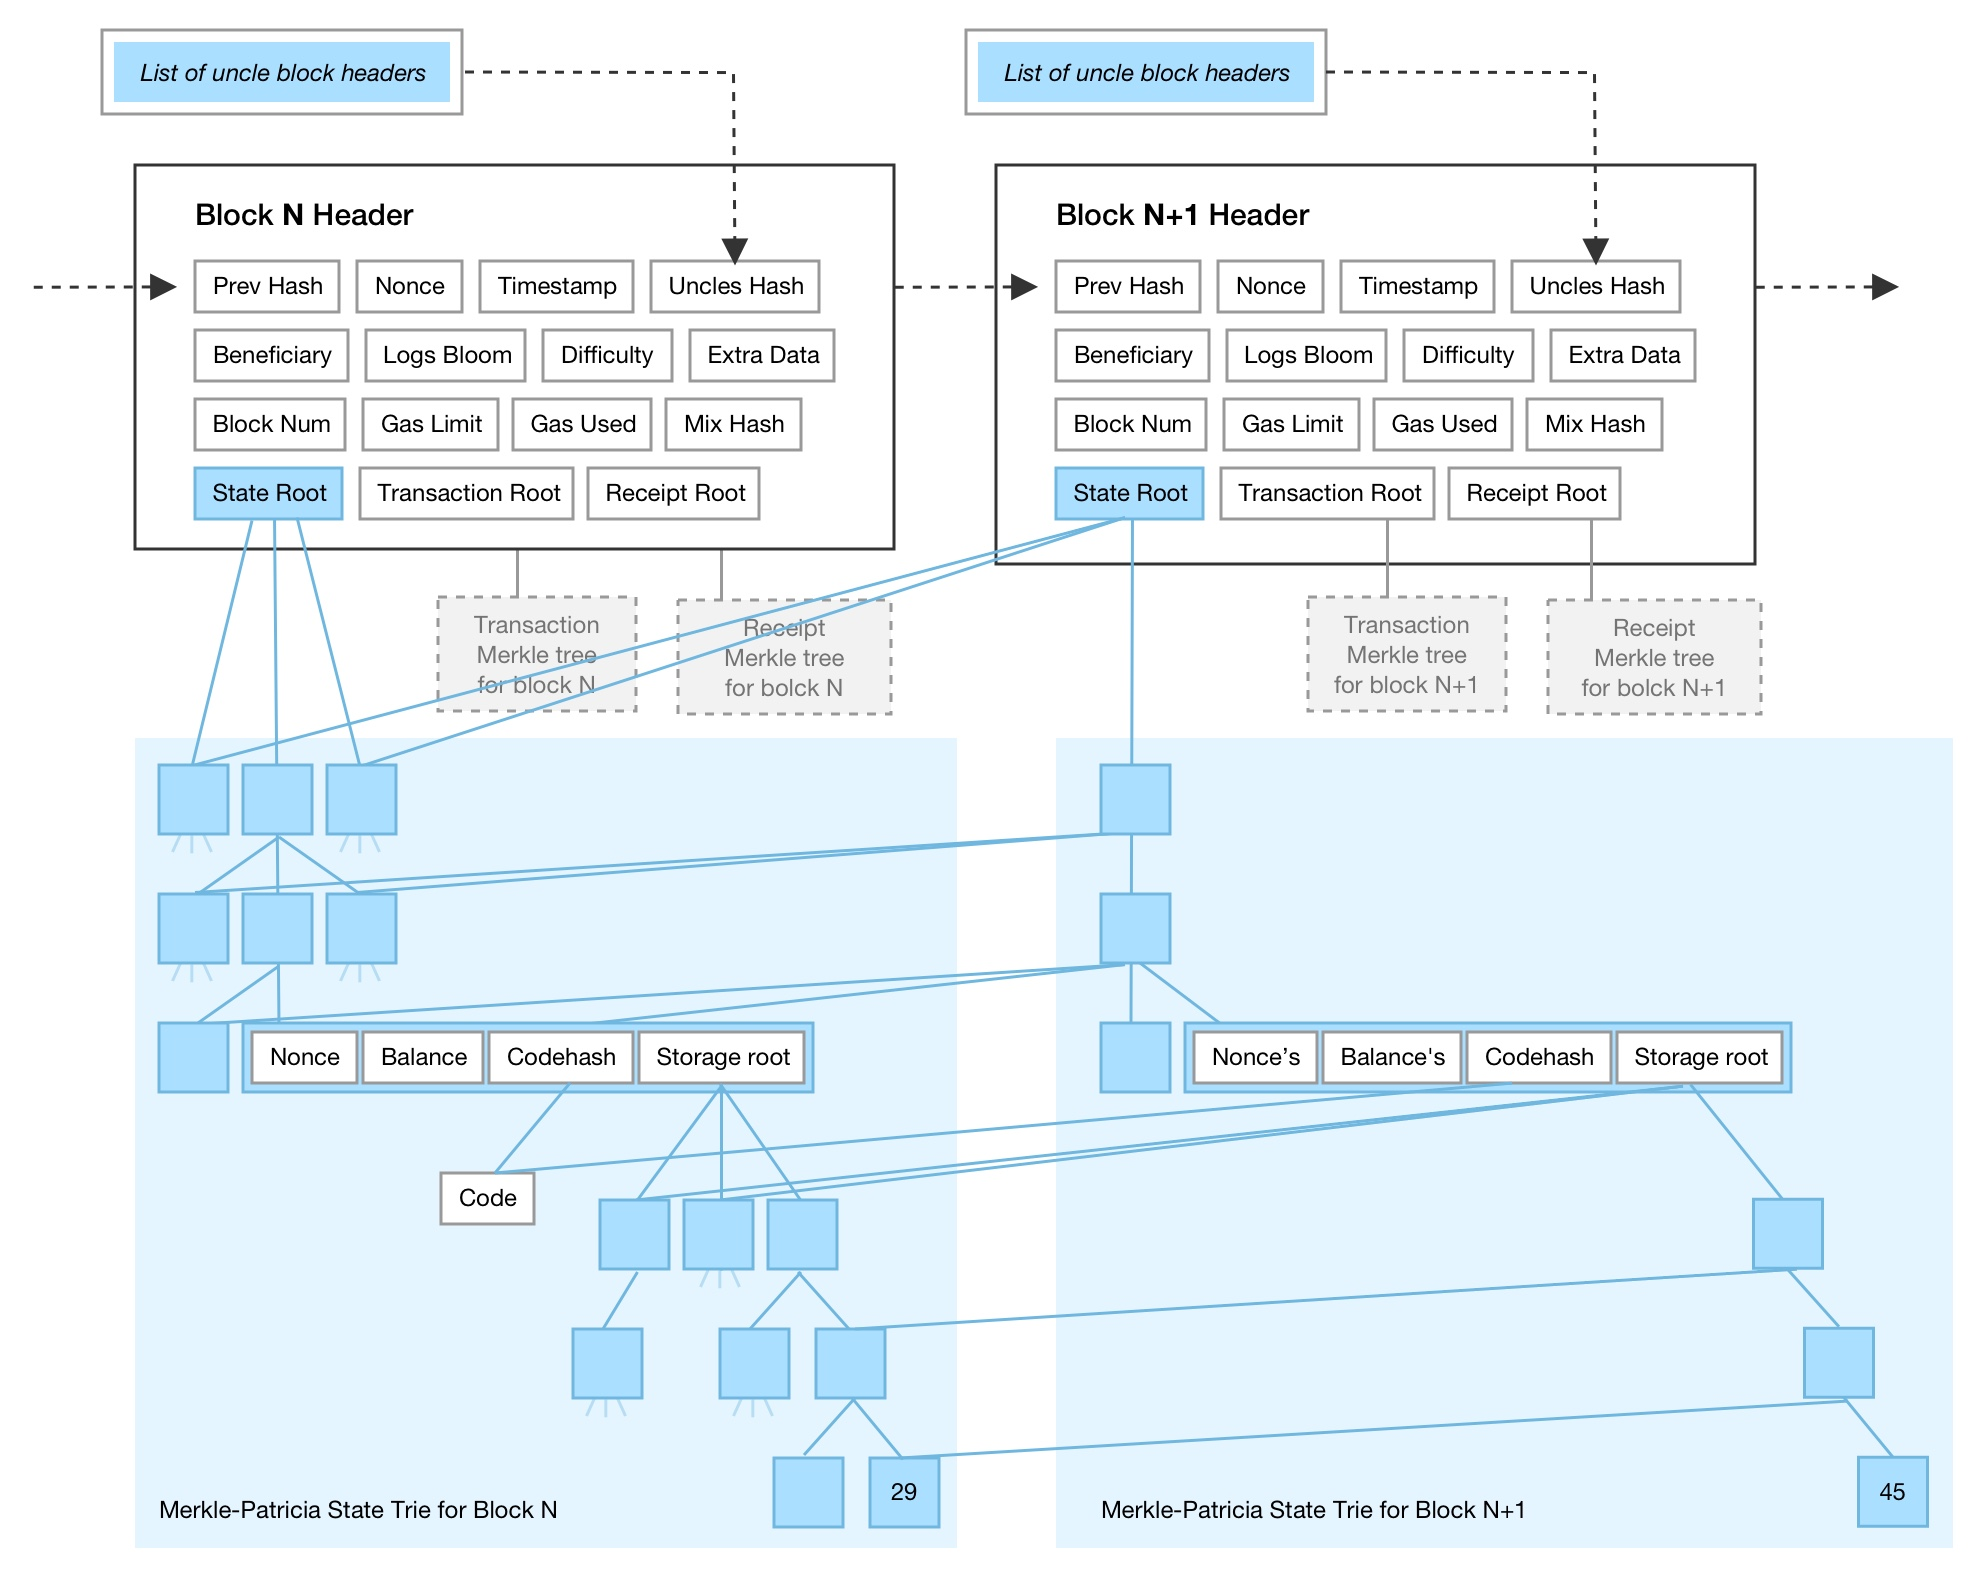
\includegraphics[scale=0.25]{pic/Merkle Patricia Tree.jpg}
\caption{Merkle Patricia Tree}
\label{fig:picture001}
\end{wrapfigure*}


\subsection*{Merkle Patricia Tree}


Merkle Patricia Tree (MPT), or Merkle Patricia Trie, is a variant structure of Merkle Tree common in Ethereum. It provides persistence and can map data (byte arrays) between binary files of arbitrary length. It is defined according to a variable data structure, mapping 256-bit binary fragments into binary data of arbitrary length. Binary data is usually stored in a database. The core of MPT and its protocol specification requirements is to provide an identifier for a given key value, which can be a 32-byte sequence or a null byte sequence. As for how to construct and implement the Trie structure efficiently, it is an implementation-level detail.


% 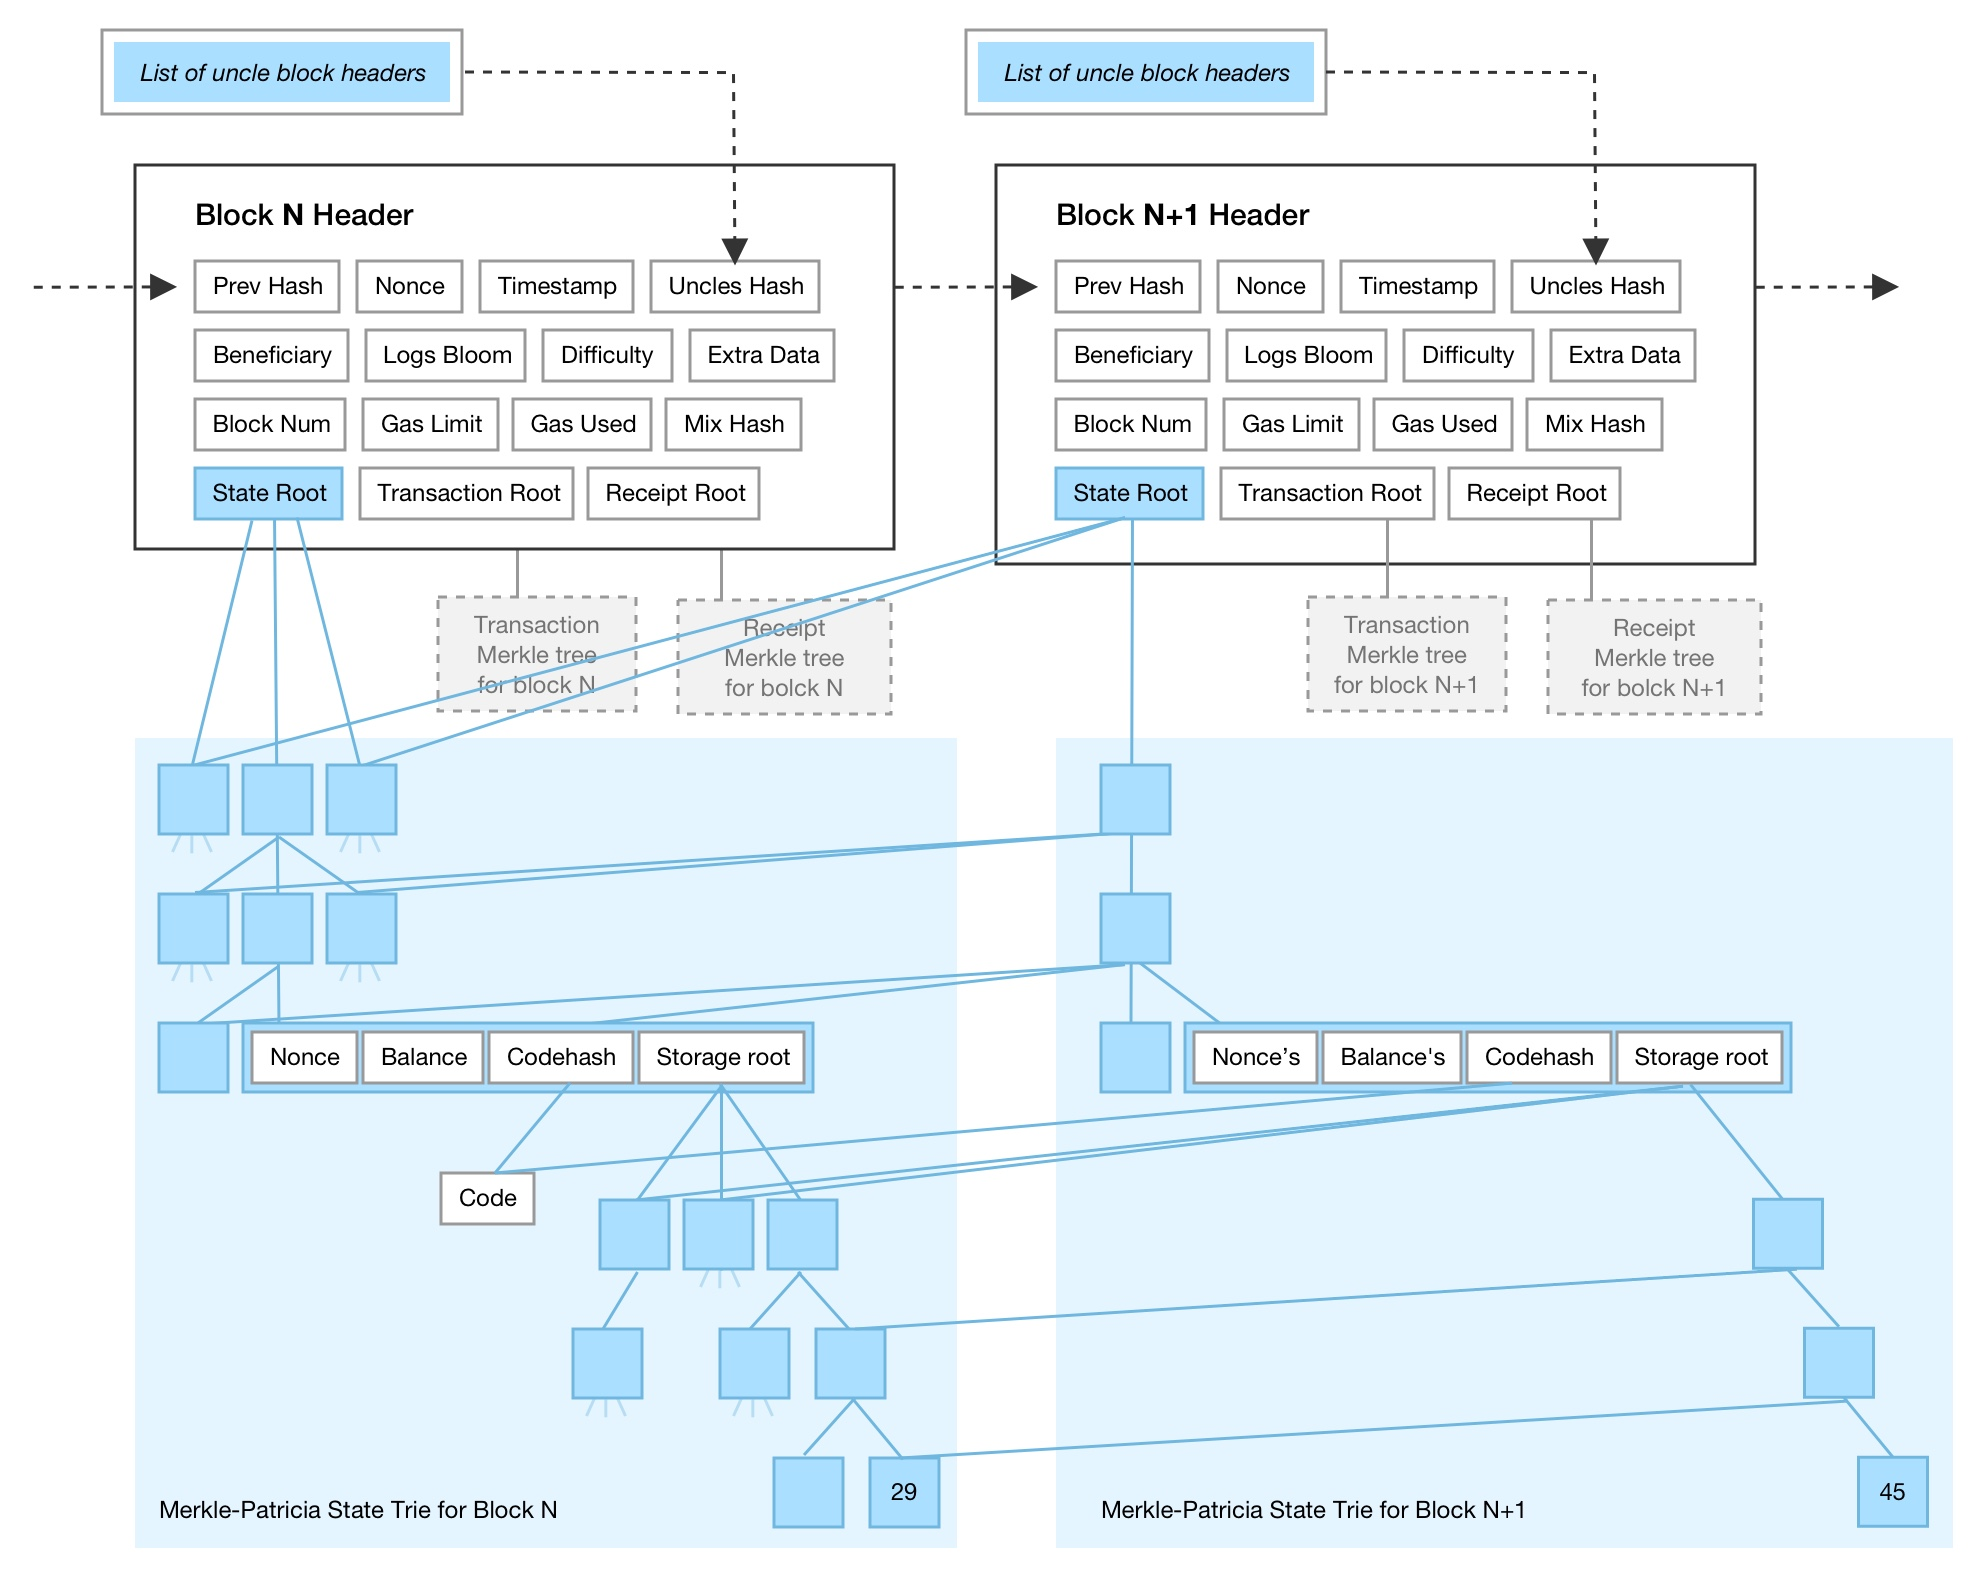
\includegraphics[scale=0.2]{pic/Merkle Patricia Tree.jpg}

Compared with Merkle Tree, the most significant advantage of MPT is that it can quickly retrieve leaf nodes. This is very useful in the state tree. When the state needs to be continuously transferred, it can maximize the reuse of existing state storage data without a frequent copy. As shown in the figure below, when a leaf node changes, most of the stored data can remain unchanged. You only need to calculate the other branch nodes and root nodes above the leaf node.